% Chapter 1

\chapter{Introducción} % Chapter title

\label{ch:introduction} % For referencing the chapter elsewhere, use \autoref{ch:introduction} 

%----------------------------------------------------------------------------------------
Durante los últimos años el incremento en el uso de Internet ha sido, se podría decir, exponencial. Diariamente nacen cientos de sitios web ofreciendo información de todos los posibles temas, desde el estado del clima hasta la imagen más reciente de nuestro vecino planeta rojo. El acceso a Internet pasó de estar en una cuantas manos, a ser usado diariamente por la mayoría de las personas en el mundo.

\marginpar{HTTP: Hypertext Transfer Protocol. Este protocolo se define por primera vez en el RFC 1945 \cite{rfc1945}. }
Uno de los principales aportes, que ayudó sin duda a la consolidación del Internet como fenómeno mundial, en la década de los noventas, fue la creación del protocolo HTTP, el cual vino a establecer una forma universal para intercambiar información. Este protocolo utiliza una arquitectura cliente-servidor, donde un cliente realiza una petición de algún recurso al servidor y el servidor satisface esta petición mediante el envió del recurso solicitado. 

Una consecuencia directa de la aceptación del protocolo HTTP en el mercado mundial fue el crecimiento de Internet. Pero esto también implicó una marcada evolución en la tecnología, pues actualmente se puede acceder a gran cantidad de información instantáneamente y la mayoría de los usuarios de Internet ignoran todo lo que esto implica. Detrás de este uso intensivo se esconde, una enmarañada red tejida de conexiones redundantes, encargadas de transportar las conexiones desde los usuarios hasta los servidores que poseen la información. 

\marginpar{ARPANET fue una de las primeras redes de conmutación de paquetes operacional producto de la guerra fría, cuando Estados Unidos quería una red de comando y control que pudiera sobrevivir una guerra nuclear \cite{Tanenbaum:2011}.} 
Por otro lado, es posible dividir Internet en dos mundos totalmente diferenciados, el primero desde su concepción, hecha en ARPANET, que fue con la idea principal de soportar cualquier desventura, y su fin es el transporte de información (capa de transporte). Y el otro mundo reside en el contenido per sé, el cual corresponde precisamente a la capa de aplicación, donde el protocolo HTTP nuevamente se hace presente como uno de los principales mecanismos de acceso a la información.

Ahora bien ¿Qué justifica esta evolución en la tecnología tanto desde el punto de vista de protocolo como de dispositivos involucrados? La respuesta es muy sencilla. Al ser HTTP un protocolo tan versátil, un lenguaje universal para el intercambio de datos, se comenzó a utilizar para diferentes aplicaciones. Se pasó de un simple intercambio de información, a ser la piedra angular por la cual se mueve la mayoría de las actividades humanas. Hoy en día tenemos muchos usos, con la aparición de la multimedia los requerimientos de todas las partes involucradas (cliente, servidor y medio de comunicación) se han incrementado. Actualmente se comparten videos de gran tamaño, se transmite televisión en alta definición, se comparte música, documentos; en fin un gran número de archivos que utilizan grandes anchos de banda, que hasta hace unos años para una conexión de 56Kbps parecía imposible.

Pero ¿Acaso esta maravilla tecnológica es gratuita? y la respuesta es no. Como se mencionó anteriormente cada parte involucrada requiere adquirir una nueva tecnología. Y es por ello que se analizará cada una de las partes involucradas en el intercambio de información, por separado. 

En el caso del cliente, es posible imaginar a una persona en su casa que renta una conexión a Internet de banda ancha para compartir archivos, revisar su correo electrónico, escuchar música, ver películas, interactuar en algún juego en línea, participar en video conferencias; y es que con estos requerimientos el equipo requerido es bastante costoso, pero se puede decir que no inaccesible. 

Ahora en el otro extremo, el servidor. Por ejemplo se supondrá un servidor que aloja un sitio web que hace transmisión de videos, los cuales son aportados por los mismos usuarios del servicio web. Ahora bien, si en este ejemplo el sitio recibiera un gran número de visitas, 100 visitas por segundo, usted como lector y experto encontraría una solución fácil al problema que supone el alto tráfico; y aumentaría el número de servidores que atienden el servicio web, además al esquema de solución se le podría agregar un balanceo de carga. Con estos previos ajustes, en efecto se puede hacer frente a este gran número de usuarios. 

\marginpar{NLB, Network Load Balancing. Consiste en el balanceo de tráfico a través de dos o más enlaces WAN sin la utilización de complejos algoritmos de enrutamiento como BGP \cite{wiki_nlb}.}
Si bien es cierto, la anterior solución es válida y en muchas ocasiones implementada. Es necesario tomar en cuenta otras variables y cuantificar todos los costos asociados, por ejemplo el precio por servidor, la solución de NLB y una conexión de Internet lo suficientemente buena como para servir videos. Unas cuantas sumas hasta aquí ya arrojarían números bastante elevados, pero lo más preocupante es que nunca es suficiente, siempre es necesario estar actualizándose, pues lo único constante es que la tecnología es cambiante y las necesidades del cliente van en aumento. 

Por otro lado, cubrir esta necesidad es una cosa, pero además de esto hay que pensar en otros riesgos asociados y que son inherentes en la publicación de un sitio en la Web por ejemplo ataques por Denegaciones de Servicio Distribuidas (DDoS), una caída del proveedor de servicios o simplemente un incremento inesperado de usuarios. Son muchas las variables que cubrir, y en todas ellas se podría decir que existen soluciones ya conocidas, pero todas implican mayor inversión por parte del individuo que desea publicar el contenido. 

Debido al problema expuesto anteriormente, aparece como solución el Caché. En su definición más sencilla podemos decir que es: "una región de memoria rápida que contiene copias de datos. El acceso a la copia en caché es más eficiente que el acceso a la original" \cite{silberschatz:2008}. 
\marginpar{Caché: "Es una región de memoria rápida que contiene copias de datos. El acceso a la copia en caché es más eficiente que el acceso a la original" \cite{silberschatz:2008}.}

En este caso en particular se podría ver como un modelo mediante el cual, objetos que se encuentran hospedados en un sitio web son almacenados en otros servidores de forma que pueden ser distribuidos desde otros servidores distintos al servidor web original, esto reduce el número de peticiones que llegan al servidor original lo que disminuye su carga (en el marco teórico de este documento se repasarán los modelos de web caché existentes). 

El caché ha sido un tema de estudio en cientos de tesis e investigaciones, pero las soluciones usadas actualmente se limitan a soluciones que deben ser adquiridas por el dueño del sitio web y como se ha discutido anteriormente, esto no es muy rentable, o bien se podrían utilizar soluciones que sean adquiridas por el cliente en su beneficio individual. Parece ser un callejón sin salida, donde la única solución es la inversión en nuevo equipo.

Por otro lado, hay otros dos aspectos de suma importancia que fueron traídos con el auge del Internet, el primero es el establecimiento de comunidades virtuales, en las cuales un grupo de Internautas se reúnen alrededor de un sitio web que presenta información de su interés y definidos como comunidad ayudan para mantenerlo, bajo un conjunto de reglas propias. 

El segundo aspecto es el compartir archivos en Internet (tal vez el más polémico de todos) y el que más le interesa a la presente investigación; es el protocolo P2P. Éste básicamente permite que un número de usuarios que cuentan con un archivo especifico lo compartan con otros de manera simultánea. Esto quiere decir que si 100 usuarios tienen un archivo de interés común y éste tiene un tamaño de 100MB, en lugar de descargarlo desde un solo servidor, descarga pequeñas partes desde cada uno de los usuarios que lo poseen, haciendo el proceso de descarga es mucho más rápido y evitando que se sature a un solo servidor.

Para ir finalizando esta introducción, el presente documento pretende proponer una posible solución de bajo costo para resolver el problema anteriormente expuesto. A esta solución se le llamó Comunidad Web Caché. 

%----------------------------------------------------------------------------------------

\section{Comunidad Web Caché}

La idea de la Comunidad Web Caché nace a partir de las siguientes premisas:

\begin{enumerate}
\item Los usuarios cuentan con una gran cantidad de recursos en sus computadoras, los cuales son desperdiciados en más de un 80\%.
\item La mayoría del contenido en Internet es de interés común y no solo de la persona que lo publica, entonces si éste es de interés común ¿Porqué solo unos cuantos deben mantenerlo?. ¿Porqué no se puede distribuir entre todos?.
\item Quien publica contenido en Internet no siempre tiene la capacidad para invertir en grandes servidores que puedan servir a un gran número de usuarios.
\item Así como existen comunidades en Internet que se conforman por un interés común, por ejemplo hacer amigos, deportes, entre otros. ¿Porqué no crear una comunidad alrededor de un sitio web?.
\end{enumerate}

La propuesta que se quiere implementar es dejar de lado el modelo tradicional de servir archivos mediante HTTP e implementar un nuevo modelo de Web Caché distinto al tradicional, utilizando las ventajas de ambos, combinado con la creación de comunidades virtuales y la utilización de los recursos de los miembros de éstas comunidades; es posible utilizar un protocolo de transferencia distribuida de contenido, en este caso P2P, para servir archivos desde diferentes localizaciones.

Basado en la figura \ref{conexionvideo} se supondrá el siguiente ejemplo: se cuenta con el sitio www.cwc.org que sirve archivos de video de más de 30Mb, con un modelo tradicional HTTP (cliente-servidor) un cliente obtendría el archivo desde un único servidor. Ahora bien, si se tienen 1000 clientes realizando esta misma operación, serían muchas solicitudes para el servidor (en el caso que éste tuviera recursos limitados), por lo tanto es necesario analizar el aumento de los recursos del servidor, entre otras cosas. 

El presente proyecto consiste en crear una comunidad alrededor del sitio anteriormente mencionado. En caso que al menos 30 de esos 1000 clientes formaran parte de la comunidad y que éstos tienen los recursos suficientes para servir archivos, entonces es posible servir los archivos en cuestión desde 31 lugares diferentes, en lugar que desde un único punto. Es evidente las ventajas que se pueden dar con un modelo como este. Ahora ¿Qué pasa si miembros de la comunidad no tienen suficientes recursos? En lugar de servir todo el archivo desde una sola localización, ese archivo se puede partir y servir desde múltiples ubicaciones, osea, que en lugar de servir archivos grandes de 30MB o más, se pueden servir sólo una porción de éstos. Esto siguiendo el concepto de una comunidad donde cada miembro aporta lo que puede, en beneficio de todos. 

\begin{figure}[h]
  \centering
    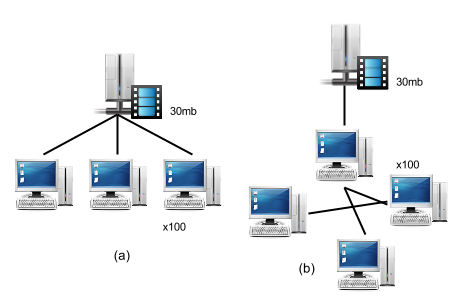
\includegraphics[scale=0.7]{gfx/conexion_video}
  \caption{Ejemplo de Conexión de Video}
  \label{conexionvideo}
\end{figure}

Otra idea podría ser que los clientes con menos recursos sirvan archivos pequeños como por ejemplo imágenes. Esto le quitaría gran cantidad de trabajo al servidor ya que una imagen significa un hilo de ejecución más que se debe crear para servir un archivo.

Uno de los objetivos es que estas comunidades se conformen de manera automática y voluntaria, esto quiere decir que un usuario instala un complemento en su navegador web y el sitio al que trata de acceder (el cual utiliza el protocolo de CWC) realiza el intercambio de manera automática sobre los archivos más relevantes que se desean mantener en caché, haciendo que éstos archivos puedan ser servidos desde la nueva ubicación dada por el nuevo miembro de la comunidad.

La cache podrá tener dos modos de operación, el primero consiste en la administración por parte del usuario, esto quiere decir que cuando el usuario accede a un contenido este queda automáticamente en la cache y el usuario puede decidir si dejarlo o eliminarlo. El segundo sería administrado por el servidor, o sea que cuando este modo se encuentra activo el servidor tendrá derecho a utilizar los recursos asignados a la caché, por lo que el servidor podrá enviar archivos que considere que deberían de estar en la caché o borrar los que no considere necesarios.

Se ampliará con mayor detalle el funcionamiento y diseño del protocolo de CWC en los siguientes capítulos.

\section{Definición del problema}

En los últimos años se ha dado un alto crecimiento en el número de usuarios de la "World Wide Web", por ejemplo a continuación se muestran las estadísticas del crecimiento de usuarios de acuerdo a el área geográfica en los últimos 10 años:

\begin{table}[h] %here h, t top, b bottom, p dedicated page on floats
\myfloatalign
\begin{tabular}{lccc} \toprule % four columns, fist left, other ones centered. 
\tableheadline{Región} & \tableheadline{2005} & \tableheadline{2010} & \tableheadline{2014}\\ \midrule
África & 2.4\% & 9.8\% & 19\% \\ 
Américas & 35.9\% & 50.5\% & 65.5\% \\
Estados Árabes & 8.3\% & 23.0\% & 40.6\% \\
Asia y Pacífico & 9.4\% & 22.5\% & 34.4\% \\
Europa & 46.3\% &	66.6\% & 74.8\% \\
\end{tabular}
\caption{Uso de Internet por Región Geográfica \citeauthor{itu:2014}.}  
\label{tab:crecimiento_internet}
\end{table}

Como se puede ver en la tabla \ref{tab:crecimiento_internet}, en casi diez años se ha duplicado o más la cantidad de usuarios de Internet, lo cual implica que se dará una mayor demanda sobre los sitios web, esto se traduce en que el dueño de un sitio web que presta un servicio deberá hacer una inversión en más recursos computacionales, como por ejemplo poder de procesamiento y ancho de banda para poder servir a sus usuarios de la mejor manera posible.

Esto quiere decir que la publicación de un sitio web con contenido de calidad no es tan trivial (se hablará en términos de contenido de calidad, ya que el contenido justificará la cantidad de usuarios que recibirá un sitio web, o sea entre mayor sea la calidad del contenido ofrecido por un sitio web para un grupo de usuarios en particular, así será la cantidad de usuarios que recibirá) ya que se deberán tomar en cuenta aspectos de crecimiento en el número de usuarios que visiten el sitio web y los requerimientos computacionales necesarios para poder prestar un servicio de calidad, acorde con los contenidos publicados.

Tomando en cuenta que realizar una publicación en Internet implica un costo para el publicador y éste se incrementa conforme aumenta el número de usuarios que soliciten los contenidos del sitio web, se podría elaborar una función de costo donde se incluyan las variables anteriormente expresadas en función de una calidad de servicio aceptable.

Este costo se traduce en que los interesados en publicar, deban de pagar por conexiones a Internet de Alta Velocidad y adquirir grandes granjas de servidores que soporten la infraestructura para hacer frente a la demanda. Es por ello que en la actualidad, solo las grandes compañías son las únicas con la capacidad de sufragar estos gastos, mediante el establecimiento de grandes caches regionales que puedan atender el tráfico generado en un área específica.

Ahora ¿Qué pasa con las pequeñas compañías, instituciones sin fines de lucro e individuos que quieren crear un sitio web con contenido de calidad y no cuentan con suficientes recursos para sufragar los gastos generados por un alto número de usuarios?. Una opción es buscar financiamiento o poner precio a sus contenidos o simplemente buscar la forma de ganar dinero mediante el bombardeo de publicidad en los sitios web, lo cual es un aspecto negativo para los usuarios.

Una vez que se han visto las necesidades de recursos computacionales para publicar contenido en Internet que es accedido por un alto número de usuarios, ¿Qué pasa con los recursos computacionales que tiene el usuario/cliente?, ¿Los recursos del cliente tienen una utilización de un 100\% en todo momento o se encuentran ociosos la mayoría del tiempo?, ya se notó que la cantidad de usuarios con acceso al World Wide Web crece enormemente, esto implica que un gran número de usuarios cuentan con una conexión a Internet con una velocidad aceptable para acceder a los contenidos de cotidianos (como videos, música, entre otros). Además también implica que cada uno de esos usuarios cuenta con una o más computadoras, las cuales obviamente cuentan con recursos computacionales aceptables para poder visualizar los contenidos ofrecidos por los sitios web, entonces se tendría la siguiente pregunta: ¿Qué sucede con todos éstos recursos de cómputo (limitado al ancho de banda, procesamiento y memoria) mientras se accede a alguna comunidad virtual, se utiliza una aplicación de ofimática, se reproduce algún contenido de multimedia en Internet o simplemente se ejecuta una aplicación de chat modo texto?  Y la respuesta es simple: se desperdician los recursos, están ociosos y están esperando a ser utilizados.

En términos de definición de la problemática, éste se encuentra compuesto por cinco partes esenciales:
\begin{enumerate}
\item Falta de recursos de quien publica contenido de calidad en Internet, esto implica un alto costo para poder atender un mayor número de clientes.
\item Un alto desperdicio de recursos en los clientes, entre estos recursos podemos citar: Ancho de Banda, Almacenamiento, Memoria y Procesamiento.
\item Una baja en la calidad del servicio conforme aumenta el número de clientes, tiempos de respuesta poco aceptables o bien se ve comprometida la continuidad del negocio. 
\item El número de usuarios en Internet se incrementa constantemente cada año, para muestra la tabla \ref{tab:crecimiento_internet}, la cual reúne el crecimiento en los últimos 10 años.
\item El problema inherente de tener un sitio con una disponibilidad del 100\%, soportando las solicitudes usuales de los clientes, las denegaciones distribuidas y las fallas en los servicios. 
\end{enumerate}

%\marginpar{¿Es posible establecer una comunidad virtual basada en una aplicación de bajo costo que utilice de una manera eficiente los recursos computacionales aportados por cada miembro y además se pueda utilizar con las aplicaciones de navegadores y servidores web utilizados actualmente?}
¿Cómo dar solución a este problema?, ¿Es posible que la solución se encuentre en una utilización eficiente de los recursos tanto del publicador cómo de los clientes?, ¿Es posible encontrar una solución de bajo costo que aproveche las causas de estos problemas para dar una solución que resuelva los problemas?, ¿Es posible el establecimiento de una comunidad virtual en la cual cada miembro de la misma, aporte un poco de recursos computacionales con el afán de mantener contenido de calidad en Internet, el cual pueda ser accedido de una forma rápida y fiable? Y aun más importante ¿Es posible establecer una comunidad virtual basada en una aplicación de bajo costo que utilice de una manera eficiente los recursos computacionales aportados por cada miembro y además se pueda utilizar con las aplicaciones de navegadores y servidores web utilizados actualmente?

\section{Justificación}

\subsection{Innovación}
%\marginpar{CWC busca establecer una comunidad en la cual cada miembro comparta un poco de sus recursos computacionales}
La Comunidad Web Caché trata de establecer una comunidad en la cual cada miembro comparta un poco de sus recursos computacionales como almacenamiento, procesamiento y ancho de banda para buscar el bien común. Esto se traduce en un incremento en la eficiencia y la velocidad del servidor web que sirve archivos.

Por otro lado, se han identificado varias problemáticas que se deben tomar en cuenta en la creación del presente proyecto y que es necesario cubrir en torno al diseño de la Comunidad Web Caché. Entre ellas se pueden mencionar:

\begin{enumerate}
\item El incremento exponencial en el número de usuarios en Internet.
\item El incremento en los recursos computacionales accesibles a los usuarios en Internet, los cuales son desperdiciados. 
\item La falta de recursos computacionales por parte de quien publica contenido de calidad en Internet, cuando aumenta el número de usuarios se vuelve un problema ya que entre más usuarios se necesitan más recursos para poder servir a estos usuarios de una manera satisfactoria.
\item La tendencia en los contenidos de moda en Internet, archivos estáticos de gran tamaño básicamente contenidos de multimedia.
\item El gran numero de comunidades con objetivos específicos que se establecen en Internet de la cual se puede tomar la decisión de formar parte.
\item La necesidad de presentar continuidad del negocio, tomando en cuenta los ataques de DDoS y tolerancia a desastres. 
\end{enumerate}
  
 
El proyecto pretende la utilización de tecnologías y productos ya establecidos, entre los cuales se tienen:

\begin{enumerate}
\item Protocolo HTTP
\item Protocolo P2P
\item Navegadores Web
\item Servidores Web
\end{enumerate}

Se podría resumir el funcionamiento de la Comunidad Web Caché como:
\begin{verse}
Quien publica contenido de calidad en Internet podrá decidir cual contenido podrá ser mantenido por la comunidad (el contenido que podrá ser mantenido por la comunidad es el que se pueda mantener en la caché, esto por el hecho de respetar el copyright). Los miembros de la comunidad podrán aportar un poco de sus recursos computacionales; es importante que ellos decidan la cantidad que aportarán. Cuando un miembro de la comunidad solicita un archivo, como un video, este será servido desde el servidor principal y desde los otros miembros de la comunidad que posean este archivo, sincronizado y previamente transferido mediante un mecanismo de P2P. Lo anterior supone que debería de incrementar la velocidad al momento de responder la solicitud, pues el archivo es seccionado y transmitido desde distintas ubicaciones, con distintos recursos y en el peor de los casos se volvería al modelo tradicional donde el archivo es distribuido desde el servidor principal. 
\end{verse}

Uno de los puntos focales del CWC es precisamente la parte comunitaria y es por ello que en el diseño se tomarán en cuenta varios conceptos propios de comunidades virtuales como: 

\begin{enumerate}
\item Aporte de recursos o participación libre: Los miembros de la comunidad decidirán qué cantidad de recursos computacionales aportaran.
\item Adhesión abierta: Puedo decidir formar parte de la comunidad o no.
\item Respeto por los contenidos privados: Se respeta el Copyright. Quien publica estos contenidos, podrá decidir si pueden ser mantenidos por la comunidad o no.
\item Bien común: los contenidos deben ser servidos de manera rápida y eficiente.
\item Apoyo: Si alguno de los miembros de la comunidad falla otro podrá tomar su lugar (tolerancia a fallos).
\end{enumerate}

En general, el CWC busca el establecimiento de una comunidad cooperativa sobre Internet utilizando los navegadores y servidores web actuales, y se diferencia de otras soluciones ya existentes. Por ejemplo, los Proxys buscan mejorar el rendimiento sobre una red de área local. 

Por otro lado, uno de los modelos más parecidos a CWC son los Proxy Federados, mejor conocidos como "Cooperative Web Caching". Éstos buscan tener un conjunto de servidores proxy que se comuniquen y que compartan los contenidos que tienen en cache sobre cualquier tipo de red, podrían utilizar en una WAN o incluso en Internet. Pero en comparación a éste último, en el CWC cualquier usuario puede formar parte de la comunidad, sin necesidad de tener que configurar un Proxy dedicado.


\subsection{Impacto}


El proyecto impactará tanto al publicador de contenido de calidad en Internet, así como a los usuarios, en los siguientes aspectos:

\paragraph{Publicador}


\begin{itemize}
\item Conforme el número de miembros de la comunidad crezca, se podrá experimentar menos carga en los servidores, por consiguiente se podrán servir muchos más usuarios.
\end{itemize}
 

\paragraph{Usuario}
\begin{itemize}
\item Conforme el número de miembros de la comunidad crezca, se podrá experimentar una utilización más eficiente de sus recursos computacionales, una mejora en los tiempos de respuesta cuando se hace una petición a un servidor web y una mayor tolerancia a fallos, dándole continuidad al negocio. 
\end{itemize}

\subsection{Profundidad}
En relación a los temas que cubrirá el presente proyecto son:
\begin{itemize}
\item Se realizará una investigación del estado del arte, en relación a los protocolos, algoritmos y mecanismo que ayuden a soportar el diseño del CWC.
\item Se realizará un levantamiento de requerimientos relacionado a las necesidades entorno a CWC.
\item Se creará un diseño completo de la implementación de CWC.
\item Se realizarán modelos que prueben el rendimiento y costos de la CWC.
\end{itemize}

Quedan fuera del alcance de este proyecto:

\begin{itemize}
\item La aplicación del protocolo de CWC en un ambiente de páginas dinámicas.
\item La aplicación del protocolo de CWC en un ambiente de flujo de video o sonido.
\item La seguridad en general, tanto del servidor como del cliente. No se especificó ningún mecanismo que permita la comprobación y la autenticidad de los elementos.
\end{itemize}

\section{Hipótesis}
El desarrollo de una caché web distribuida que permita compartir de manera transparente y eficiente los recursos computacionales distribuidos ofrecidos colaborativamente mediante una comunidad de servidores, tendrá un impacto positivo en el bajar los costos y mejorar la continuidad del negocio para las comunidades virtuales.

\section{Objetivos}
\subsection{Objetivo Principal}
Desarrollar una caché web distribuida que permita compartir de manera transparente y eficiente los recursos computacionales distribuidos ofrecidos colaborativamente mediante una comunidad de servidores.

\subsection{Objetivos Específicos}
\begin{itemize}
\item Compilar y comparar trabajos relevantes relacionados con sistemas distribuidos
\item Examinar las oportunidades de mejoramiento estratégico de las plataformas existentes.
\item Determinar los requerimientos de la caché web distribuida basada en HTTP.
\item Diseñar una arquitectura de una caché web distribuida bajo un conjunto de principios tales como: transparencia de ubicación de los recursos, solución de bajo costo y calidad de servicio.
\item Desarrollar un prototipo de la caché web distribuida.
\item Analizar el rendimiento de velocidad y el costo del entorno de CWC.
\end{itemize}

\section{Alcances}

\begin{itemize}
\item Investigación del funcionamiento de Protocolos P2P y HTTP.
\item Investigación de los diferentes modelos de caching existentes con el fin de identificar sus características, arquitectura, funcionamiento, debilidades y fortalezas. Esto ayudará en una etapa posterior para realizar el diseño de la Comunidad Web Caché.
\item Investigación sobre el establecimiento de comunidades virtuales y las implicaciones de estas.
\item Investigación  a soluciones que utilicen los diferentes modelos de web caching, esto permitirá tener un punto de comparación para nuestros modelo y establecerá los umbrales a mejorar.
\item Investigación de modelos de consistencia.
\item Elaboración del diseño del CWC el análisis de las investigaciones previas. Este modelo se limitará únicamente a contenido estático y no se desarrollará el diseño para la compatiblidad de contenido dinámico y contenidos de flujo de video o sonido, los cuales implican modelos de consistencia mucho más complejos, además de algoritmos de reemplazo y muchas otras implicaciones de diseño que necesitan de una investigación aún mayor.
\item Elaboración de prototipo de sistema para compartir archivos de manera distribuida tomando en cuenta ciertas partes del diseño. Este prototipo pretende convertirse en la base para el desarrollo del CWC.
\end{itemize}

\section{Entregables}
\begin{enumerate}
\item Informe investigación funcionamiento de protocolo HTTP.
\item Informe investigación funcionamiento de protocolo P2P.
\item Informe investigación de modelos de Web Caché existentes.
\item Informe investigación sobre comunidades virtuales.
\item Informe investigación de aplicaciones que utilicen los diferentes modelos de Web Caché.
\item Informe investigación de modelos de consistencia.
\item Documento de requerimientos de Comunidad Web Caché.
\item Prototipo de CWC Cliente.
\item Prototipo de CWC Server.
\item Análisis de rendimiento de velocidad del entorno de CWC.
\item Análisis de costos del Entorno de CWC.
\end{enumerate}  

%----------------------------------------------------------------------------------------